
The system used in the experiment is composed by a non-anthropomorphic platform and software architecture that enrich robot's movements with emotion. The robotic platform was envisioned to be as simple as possible to limit the influence of shape on the study of the desired characteristics. 

%%%%%%%%%%%%%%%%%%%%%%%
\subsection{Hardware and Mechanical}

A holonomic platform was built to be used in the experiment. This type of platforms are characterized by the possibility to move in any direction without the necessity to have a specific orientation, i.e., they are free to move taking any desired orientation. Therefore, it was possible to imitate movements that are done by humans. For example, people do not have constaraints in movement, and can take any direction in any moment. The platform has a diameter of 25 cm and height of 25 cm. Figure~\ref{fig:ThirdDesign} shows the platform's blue prints and the real platform. Robot's frame of reference, in which all the velocities are going to be calculated, is depicted by the two black arrows. So, as it could be observed, to make the robot move forward a velocity along the $y$ axis is selected by the control system.

\begin{figure}
	\centering
	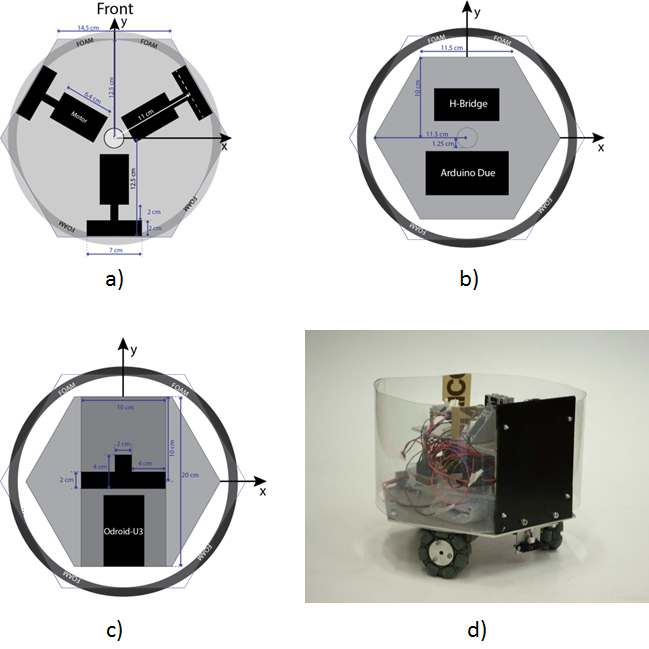
\includegraphics[width=0.48\textwidth]{Images/DesignThird.png} 
	\caption{Design of the platform. a) Base platform, this layer is used to carry the batteries. The two black arrows represent robot's frame of reference. b) First layer, which includes Arduino and the H-Bridges to control the motors. c) Second layer with Odroid-U3 and the mechanical structure to support the upper part. d) Lateral view of the robot.}
	\label{fig:ThirdDesign}
\end{figure}

%%%%%%%%%%%%%%%%%%%%%%%platform_base
\subsection{Software}
To guarantee that the correct robot's velocity for each motor could be achieved, a PID controller was implemented. PID's set point is established by a higher level controller that could receive two different types of commands. The first commands are robot's velocities ($<V_x,V_y,\omega>$), given in robot's reference frame. The second command is a set point ($<x, Y, \theta>$) to be reached, given in the world reference frame. This frame of reference is set every time the system is reset or boot. For example, if the robot finishes a trajectory and then it is reset, the new frame is going to be in the robot's current position.  %TODO From this description it seems that this second reference frame is again associated to the robot, in particular that it is a reference frame that is activated when the robot starts, and does not move with the robot. So it is a world reference frame reset each time the robot starts a new movement. It should have a name, to be found. If it was always associated with the robot it would have been called "deictic".

%TODO I'm sorry, but the following is an implementation detail that does not add anything to the scientific relevance of this paper, and this is not a paper about the interface.
%In addition to this low level control, a graphical interface, depicted in Figure~\ref{fig:experimental_interface}, was created to reduce the possibility of introducing wrong values for a desired sequence. This interface loads the sequences from a .txt file and displays sequences' numbers on it. Every time that a new sequence should be presented to a participant, the sequence's number is selected in the interface, which will display sequence's values. Once the robot has been positioned to the correct position, the execution could be started by clicking on send button. Here two commands are send, one resetting the controller and the second the desire position. In case that the sequence's execution should be aborted, it should be clicked the button stop.

%\begin{figure}
%	\centering
%	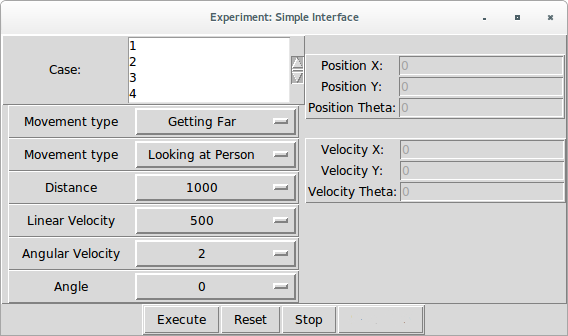
\includegraphics[width=0.45\textwidth]{./Images/ExperimentInterface.png} 
%	\caption{Interface used in the experiment. Once a sequence is selected, the interface shows sequence's values. Also, the interface give information about the current position of the robot and its velocity.}
%	\label{fig:experimental_interface}
%\end{figure}